\documentclass[a4paper,12pt]{article}

\usepackage{amsmath,amsthm,amssymb,ae,aecompl,sgame,natbib,sgamevar}
\usepackage[margin=2.5cm]{geometry}
\usepackage{tikz}
\usetikzlibrary{trees}

\title{Exercises Adv. Micro II}
\author{Christoph Schottm\"uller}

\begin{document}

\maketitle

\section{Rationalizability}
\begin{enumerate}
\item %Come up with a three player game in which each player has two actions and the actions surviving iterative elimination of strictly dominated strategies is not the same as the set of rationalizable actions.
  Show that in the following three player game (only payoffs of player 1 are given), $M$ is a never best response although $M$ is not strictly dominated.
\begin{table}[h]
    \centering
    \begin{tabular}{l|c|c}
      & L &R\\ \hline
      U& 10,  &10, \\
      M&6,  &0, \\
      D& 0, & 10,
    \end{tabular}
    $\qquad$
    \begin{tabular}{l|c|c}
      & L &R\\ \hline
      U& 10,  &0,  \\
      M&0,&6, \\
      D& 10, & 10,
    \end{tabular}
    \caption{P1 chooses row, P2 column, P3 table}
    \label{tab:domVsRatio}
  \end{table}
  
\item Show that the order of elimination does not matter for the outcome of iterative elimination of strictly dominated strategies. \\(Hint: Consider two orders, say A and B, and suppose they lead to different outcomes. Consider then the first action to be deleted in one procedure, say A, while surviving the other, i.e. B. Show that this action is strictly dominated at the end of procedure B which yields the desired contradiction.)
\item (Numerical) Consider two players participating in a lab experiment. The monetary payoffs the two players get from the experimenter when choosing their strategies are given in table \ref{tab:monRatio}. (note: this time the numbers in the table are not utilities but amounts of money!) Assume that players are only interested in their own monetary payoffs and not in the monetary payoffs for the other players.
  \begin{table}[h]
    \centering
    \begin{tabular}{l|c|c}
      & L &R\\ \hline
      U& 3,1  &0,0  \\
      M1&1,0&1,1 \\
      M&2.6,0  &0.5,0 \\
      D& 0,1 & 3,0
    \end{tabular}
    \caption{Monetary payoff}
    \label{tab:monRatio}
  \end{table}
  \begin{enumerate}
  \item Suppose players value money linearly $u_i(x)=x$ for any monetary amount $x$. Which actions are rationalizable?
  \item Suppose players value money  $u_i(x)=-e^{-r x}$ for any monetary amount $x$. Which actions are rationalizable if the parameter $r$ is very high? (you can choose a high number like $3$ and check)
     \item Suppose players value money $u_i(x)=e^{r x}$ for any monetary amount $x$. Which actions are rationalizable if the parameter $r$ is very high?
     \end{enumerate}
     What is the interpretation in terms of risk preferences? (see \cite{weinstein2016effect} for more on this topic)
\end{enumerate}


\section{Existence of Nash equilibrium}
\label{sec:nash-theorem-fixed}

\begin{enumerate}
\item Show that a pure strategy Nash equilibrium exists in the following two player game: $I=\{P1,P2\}$, $S_1=S_2=[0,1]$, $u_i(s_i,s_{-i})$ is differentiable and strictly (quasi-)concave in $s_i$ and $\partial u_i/\partial s_i$ is continuous in both variables.\\
  (Hint: Show that the first order condition leads to a continuous best response function. Then, verify that the two best response functions must intersect.)
\end{enumerate}

\section{Correlated equilibrium}
\label{sec:corr-equil}
\begin{enumerate}
\item Find a correlated equilibrium that yields a higher payoff to every player than the unique Nash equilibrium (game in table \ref{tab:corEq}).
   \begin{table}[h]
\centering
 \begin{game}{3}{3}
       \> L \> C \>R\\ %\hline
U   \>1,1   \> 2,4 \> 4,2   \\
M   \>4,2   \> 1,1 \> 2,4 \\
D  \> 2,4    \>4,2  \>1,1
\end{game}  
\caption{correlated equilibrium}
\label{tab:corEq}
\end{table}
\item In the example from the lecture (using in particular the inequalities on slide 9), show that the set of correlated equilibria is the set of all probability distributions $(p_{UL},p_{UR},p_{DL},p_{DR})$ for which the the probability on each pure Nash equilibrium is at least as high as the probability on any other strategy profile. (Note: This is \emph{not} a general result!) Given this, derive the correlated equilibrium with the lowest and the highest sum of payoffs. 
\end{enumerate}

\section{Bayesian Nash equilibrium}
\label{sec:Bayes-nash-eq}
\begin{enumerate}
\item Two player Cournot with uncertain costs: Payoffs of player $i$ are $(\theta _i-q_1-q_2)q_i$ where $\theta _i$ is the difference between the intercept of a linear demand function and costs. It is commonly known that $\theta _1=1$. However, $\theta _2$ is private information of firm 2. Firm 1's (commonly known) belief is that $\theta _2$ is $3/4$ with probability $1/2$ and $5/4$ with probability $1/2$.
  \begin{enumerate}
  \item If firm 1's equilibrium quantity is $q_1^*$, what is firm 2's best response?
  \item If type $j\in\{l,h\}$ of firm 2 produces quantity $q_2^j$, what is firm 1's best response quantity? (i.e. maximizing expected payoff)
    \item What is the BNE of this game?
  \end{enumerate}
\item Purification: Consider the game in table \ref{tab:purify}. Let $\theta _i$ be private information and be distributed uniformly on $[0 ,\varepsilon ]$. Assuming $\varepsilon >0$ sufficiently small, derive a BNE in cutoff strategies; i.e. P1 (P2) plays U (L) if $\theta _1>\bar{\theta }_1$ ($\theta _2>\bar{\theta }_2$) and D (R) otherwise for some $\bar \theta_i\in(0,{\varepsilon })$. Compare the equilibrium in the limit as $\varepsilon \rightarrow 0$ to the mixed strategy equilibrium in the game without private information (i.e. the game where $\theta _i=0$ is commonly known). 
     \begin{table}[h]
\centering
 \begin{game}{2}{2}
       \> L  \>R\\ %\hline
U   \>5$+\theta_1$,1$+\theta _2$    \> $\theta_1$,0   \\
D  \> 4,4$+\theta _2$    \>1,5
\end{game}  
\caption{purification}
\label{tab:purify}
\end{table}
\end{enumerate}

\section{Auctions}
\label{sec:auctions}

\begin{enumerate}

\item Take the first price sealed bid auction in the independent private value framework. The purpose of this exercise is to show that in every BNE, the bidding strategy of an arbitrary bidder $i$ is weakly increasing in his valuation. Take two values $v_i^h$ and $v_i^l$ with $v_i^h>v_i^l$ and let $s_i()$ be an equilbrium strategy of player $i$.
  \begin{enumerate}
  \item In equilibrium type $v_i^l$ must prefer bidding $s_i(v_i^l)$ to bidding $s_i(v_i^h)$. Write down the corresponding inequality.
    % (v_i^l-s_i(v_i^l))*prob(win,s_i(v_i^l))\geq (v_i^l-s_i(v_i^h))*prob(win,s_i(v_i^h))
  \item In equilibrium type $v_i^h$ must prefer bidding $s_i(v_i^h)$ to bidding $s_i(v_i^l)$. Write down the corresponding inequality.
    % (v_i^h-s_i(v_i^h))*prob(win,s_i(v_i^h))\geq (v_i^h-s_i(v_i^l))*prob(win,s_i(v_i^l))
  \item Use the two inequality to show that $s_i(v_i^h)\geq s_i(v_i^l)$. (Hint: Note that bidding higher increases the probability of getting the object in a first price auction!)
    % adding inequalities gives: $(v_i^h-v_i^l) (prob(win,s_i(v_i^h))-prob(win,s_i(v_i^l))\geq 0$ which is only true if $s_i(v_i^h)\geq s_i(v_i^l)$
  \end{enumerate}
  
% \item Two people have to decide who gets an indivisible item. Their valuations of the item are private information and we regard the two $v_i$ as drawn independently from a uniform distribution on $[0,1]$. The two people have come up with the following auction mechanism: They simultaneously state a bid $b_i$ and the one stating the higher bid gets the item but has to pay half of his bid to the other player.
%   \\
%   Assume that there is a symmetric equilibrium of this game in which players bid according to a strictly increasing strategy $s(v)$. (If you find this hard, assume that $s(v)=\alpha v$ for some $\alpha>0$ and determine below the $\alpha$ for which this is an equilibrium.)
%   \begin{enumerate}
%   \item Write down the expected payoff of a player bidding $b$ (given that the other player bids according to $s$). (Hint: Do not forget that he might receive a payment from the other player!)
%     % $\int_0^{t(b)}v_i-b/2 \,dv_j+\int_{t(b)}^1 s(v_j)/2\,dv_j$
%   \item Derive the first order condition of an optimal bid.
%     % $t'(b)(v_i-b/2)-t(b)/2-t'(b) b/2=0$
%   \item What is the equilibrium bidding strategy? Why is it not optimal to bid your true valuation?
%     % use $t(b)=v_i$, $b=s(v_i)$ and $t'(b)=1/s'(v_i)$ in foc to get $(v_i-s(v_i))/(s'(v_i))-v/2=0$ which is solved by $s(v_i)=v_i*2/3$
%   \end{enumerate}
\item A buyer's valuation is uniformly distributed on $[0,1]$ and the buyer's private information. A seller's cost is also uniformly distributed on $[0,1]$ and the seller's private information. The buyer states an ask price $b_b$ and the seller simultaneously states an offer price $b_s$. If $b_s<b_b$, trade takes place at price $(b_s+b_b)/2$ while otherwise trade does not take place.
  \begin{enumerate}
  \item Explain/show why $b_s(c)=c$ and $b_b(v)=v$ is not an equilibrium although it would maximize welfare. 
  \item Show that the following is an equilibrium for any given $p\in[0,1]$:
    \begin{equation*}
      b_b(v)=
      \begin{cases}
        p & \text{ if }v\geq p\\
        0 & \text{ else }
      \end{cases}
    \qquad
      b_s(c)=
      \begin{cases}
        p & \text{ if }c\leq p\\
        1 & \text{ else }.
      \end{cases}
    \end{equation*}
    \item Suppose that players use linear strategies $b_b(v)=\alpha+\beta v$ and $b_s(c)=\gamma+\delta c$ with $\beta,\delta>0$. Taking the strategy of the other player derive the best response of a seller/buyer with valuation $v$ / cost $c$. For which values of $\alpha,\beta,\gamma,\delta$ form the linear strategies an equilibrium?
    \end{enumerate}
  \item Two players participate in a contest: Each player chooses an effort level $e_i$. Effort is costly and reduces player $i$'s payoff by  $\theta _ie_i$. The player who choose the highest effort wins a prize of value 1. That is, the winner has payoff $1-\theta _i e_i$ while the loser has payoff $-\theta _i e_i$. The $\theta _i$ are private information and each player views the other player's type as being uniformly distributed on $[0.1,1.1]$. \\
    Write player $i$'s maximization problem given that the other player uses a strictly decreasing strategy $s$ (with inverse $t$). Derive the first order condition for optimal effort choice. Solve for a symmetric equilibrium in strictly decreasing strategies.
    % $\max_{e}(1.1-t(e))-\theta _i e$ where $t$ is the inverse of the other player's strategy $s$. Foc: $-t'(e)-\theta _i=0$, in equilibrium $t'(e(\theta _i))=1/s'(\theta _i)$ and we get $s'(\theta _i)=-1/\theta _i$. Using $s(1.1)=0$, we get $s(\theta _i)=\int_{\theta _i}^{1.1}1/x \,dx=log(1.1)-log(\theta _i)$
    (More on such contests can be found in \cite{moldovanu2001optimal}.)
\end{enumerate}

\section{Subgame perfect Nash equilibrium}
\label{sec:subgame-perfect-nash}

\begin{enumerate}
\item $I$ Players play the same strategic form game $\Gamma=[I,\{S_i\},\{u_i\}]$ $T$ times. Players observe immediately after each round $t=1,\dots, T$ which actions were chosen by the other players. Assume that $\Gamma$ has a unique Nash equilibrium $\sigma$. Show that the extensive form game $\Gamma_E$ formed by the $T$ time repetition of $\Gamma$ has a unique subgame perfect Nash equilibrium. (extra exercise: find an example $\Gamma$ with a unique NE in which $\Gamma_E$ has several NE that are not subgame perfect.)
  % add a "total destruction" action yielding for both players -1000 to a normal prisoner's dilemma and let $T=2$; the strategy cooperate in 1; defect in 2 if cooperation in 1 and total destruction otherwise is a NE but not subgame perfect
\end{enumerate}

\section{Weak PBE and sequential equilibrium}
\label{sec:weak-pbe-sequential}

\begin{enumerate}
\item Find a pure strategy NE in the game of figure \ref{fig:selten_ex}. Show that this NE is subgame perfect but not sequentially rational. Find a weak PBE. (Hint: use mixed strategies)
   \begin{figure}[h]
\centering
% First, set the overall layout of the tree
% You might need to play with these sizes to ensure nothing overlaps.
\tikzstyle{level 1}=[level distance=1.5cm, sibling distance=6cm]
\tikzstyle{level 2}=[level distance=1.5cm, sibling distance=2.5cm]
\tikzstyle{level 3}=[level distance=1.5cm, sibling distance=2cm]
\tikzstyle{level 4}=[level distance=1.5cm, sibling distance=1.5cm]
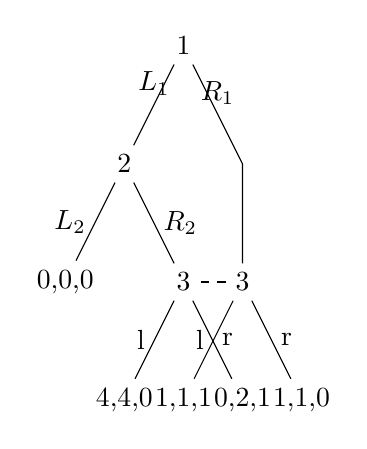
\begin{tikzpicture}
%Start with the parent node, and slowly build out the tree
% with each "child" representing a new level of the diagram
% each "node" represents a labelled (or unlabeled if you 
% want) node in the diagram.
\node{1}
    child{
             node{2}
             child{
               node{0,0,0}
             edge from parent
             node[left]{$L_2$}}
             child{
               node(b){3}
                  child{
               node{4,4,0}
               edge from parent
               node[left]{l}
               }
             child{
               node{0,2,1}
               edge from parent
               node[right]{r}
               }
                edge from parent
                node[right]{$R_2$}
               }
           edge from parent
           node[left,above]{$L_1$}
           }
    child{
           child{
               node(c){3}
                  child{
               node{1,1,1}
               edge from parent
               node[left]{l}
               }
             child{
               node{1,1,0}
               edge from parent
               node[right]{r}
               }
               }
         edge from parent
         node[right,above]{$R_1$}
         };
\draw [dashed](c)--(b);
\end{tikzpicture}
\caption{Selten's horse}
\label{fig:selten_ex}
\end{figure}

\item Consider the two games in figures \ref{fig:seq_eq_coalescing} and \ref{fig:seq_eq_coalescing2}. To what extent are these games different or the same? Show that there is a pure strategy sequential equilibria in figure \ref{fig:seq_eq_coalescing} that does not exist in \ref{fig:seq_eq_coalescing2}. Would this also be true for  weak PBE instead of sequential equilibrium?
% (R,r) supported by belief (0,1) is seq eq in first game but there is no equivalent in the second as A strictly dominates B and therefore seq rationality requires P1 to play A instead of B in the subgame. For any completely mixed strat converging to ?A P2's belief must be (1,0) and therefore his action in seq eq is l which means (LA,l) is unique seq eq in second game. Note that (RA,r) with belief (0,1) is still a weak PBE as P2's info set in never reached.
  
   \begin{figure}[h]
\centering
% First, set the overall layout of the tree
% You might need to play with these sizes to ensure nothing overlaps.
\tikzstyle{level 1}=[level distance=1.5cm, sibling distance=3.5cm]
\tikzstyle{level 2}=[level distance=1.5cm, sibling distance=1.5cm]
\tikzstyle{level 3}=[level distance=1.5cm, sibling distance=2cm]
\tikzstyle{level 4}=[level distance=1.5cm, sibling distance=1.5cm]
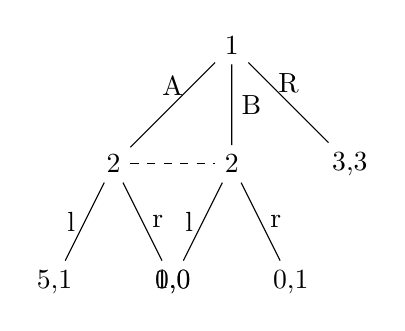
\begin{tikzpicture}
%Start with the parent node, and slowly build out the tree
% with each "child" representing a new level of the diagram
% each "node" represents a labelled (or unlabeled if you 
% want) node in the diagram.
\node{1}
             child{
               node(a){2}
                  child{
               node{5,1}
               edge from parent
               node[left]{l}
               }
             child{
               node{1,0}
               edge from parent
               node[right]{r}
               }
               edge from parent
               node[left,above]{A}
               }
             child{
               node(b){2}
                  child{
               node{0,0}
               edge from parent
               node[left]{l}
               }
             child{
               node{0,1}
               edge from parent
               node[right]{r}
               }
               edge from parent
               node[right]{B}
               }
    child{
         node{3,3}
         edge from parent
         node[right, above]{R}
         };
\draw [dashed](a)--(b);
\end{tikzpicture}
\caption{sequential equilibrium and coalescing moves}
\label{fig:seq_eq_coalescing}
\end{figure}

 \begin{figure}[h]
\centering
% First, set the overall layout of the tree
% You might need to play with these sizes to ensure nothing overlaps.
\tikzstyle{level 1}=[level distance=1.5cm, sibling distance=3.5cm]
\tikzstyle{level 2}=[level distance=1.5cm, sibling distance=3.5cm]
\tikzstyle{level 3}=[level distance=1.5cm, sibling distance=2cm]
\tikzstyle{level 4}=[level distance=1.5cm, sibling distance=1.5cm]
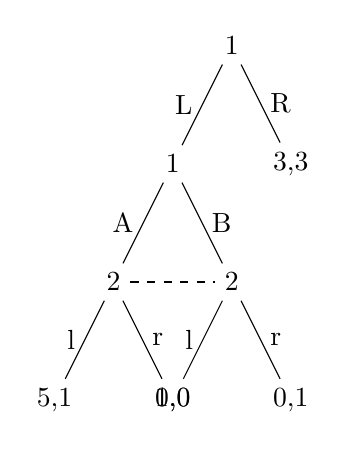
\begin{tikzpicture}
%Start with the parent node, and slowly build out the tree
% with each "child" representing a new level of the diagram
% each "node" represents a labelled (or unlabeled if you 
% want) node in the diagram.
\node{1}
    child{
             node{1}
             child{
               node(a){2}
                  child{
               node{5,1}
               edge from parent
               node[left]{l}
               }
             child{
               node{1,0}
               edge from parent
               node[right]{r}
               }
               edge from parent
               node[left]{A}
               }
             child{
               node(b){2}
                  child{
               node{0,0}
               edge from parent
               node[left]{l}
               }
             child{
               node{0,1}
               edge from parent
               node[right]{r}
               }
               edge from parent
               node[right]{B}
               }
           edge from parent
           node[left]{L}
           }
    child{
         node{3,3}
         edge from parent
         node[right]{R}
         };
\draw [dashed](a)--(b);
\end{tikzpicture}
\caption{game above with additional move}
\label{fig:seq_eq_coalescing2}
\end{figure}

\end{enumerate}

\section{Signaling}
\label{sec:signaling}

\begin{enumerate}
% \item Take the jobmarket model from the slides. Suppose that the worker has an outside option, i.e. if he is offered only wages of less than $r>0$, than he will refuse all offers and take his outside option (of value $r$). The value of the outside option does not depend on type. What are the equilibria if $r\in(\theta_l,\mathbb{E}[\theta]$? What are the equilibria if $r>\mathbb{E}[\theta ]$? How do you evaluate the welfare effect of the possibility to signal?
\item Consider the least cost separating equilibrium of the jobmarket model on the slides. Suppose the government introduces a tax on high wages (all wages above $\mathbb{E}[\theta ]$) and a subsidy for low wages (all others). The tax is $t$ and the subsidy is $t*\lambda/(1-\lambda)$, i.e. the tax subsidy scheme has a balanced budget. Show that this (i) tax scheme leads to a Pareto improvement if $\lambda$ is sufficiently large (and $t$ is chosen not too large) and (ii) high productivity types are worse off as a result of the tax if $\lambda$ is low. 
  % Firms always get zero profits and $\theta_l$ types clearly are made better off by the subsidy.  A marginal increase in $t$ from $t=0$ improves welfare of high types if their cost of effort is reduced by more than the tax burden. The marginal effect of the tax on payoff is $-1$. The reduction in effort (at $t=0$) is determined from the indifference condition $\theta_h-t-c(e,\theta _l)=\theta _l+t\lambda/(1-\lambda)$ via implicit function theorem, i.e. $d\tilde e/dt=-1/((1-\lambda)*c_e(\tilde e,\theta_l))$. Hence, welfare of $\theta_j$ goes up by $\frac{1}{1-\lambda}\frac{c_e(\tilde e,\theta_h)}{c_e(\tilde{e},\theta _l)}$. For $\lambda$ sufficiently close to 1 this is higher than 1, for $\lambda$ sufficiently close to zero it is less than 1 by the single crossing assumption. 
\item Exercise 13.C.6 in MWG.
\end{enumerate}

\section{Cheap talk}
\label{sec:cheap-talk}

\begin{enumerate}
\item The state of the world $\theta $ is either 0 or 1. Both, 0 and 1, have probability 1/2. An expert observes the state and then sends a cheap talk message to a decision maker. The available messages are ``high'' (h) and ``low'' (l). (Assume in the following that the messages are used in accordance with their name, i.e. the high message leads to a higher belief of the decision maker.) The decision maker chooses an action $a\in [0,2]$ with the objective of maximizing $-(a-\theta )^2$. The objective of the expert is $-(a-\theta-b)^2$ for some $b\in(0,1)$.
  \begin{enumerate}
  \item What is a mixed strategy for the expert? % probability of sending high message for each state
    \item Intuitively, which state will the expert reveal truthfully? % high state as expert always wants higher action than DM
    \item Given a mixed strategy of the expert, what are the decision maker's beliefs when receiving a low/high message? % in state 0, let prob of h be q (while in state 1 it is 1), then $mu(l)=0$ and $\mu(h)=\frac{.5*1}{.5*1+0.5*q}=1/(1+q)$
      \item Given a mixed strategy of the expert, what is the best response of the decision maker? % $min \mu * (a-1)^2+(1-\mu)(a)^2$ which gives foc: $a=\mu$ 
      \item What is the equilibrium strategy of the expert? %truthtelling is eq if $-b^2\geq-(1-b)^2$, i.e. if $b\leq 1/2$; otherwise indifference of expert in 0 state: $b^2=(1/(1+q)-b)^2$ solved for $q=1/2b-1$ which is eq also for b<1/2; otherwise babbling
      \end{enumerate}
    \item Take the model from the lecture but assume that the state is distributed not uniformly but with some arbitrary distribution $\Phi$ (with strictly positive density $\phi$) on $[0,1]$. Take a partitional equilibrium as in the lecture. Show that $a(m)=\mathbb{E}[\theta |m]$. Show then that S benefits from commitment in expectation, i.e. if S could commit to always truthfully reveal the state he would in expectation be better off than in equilibrium (where the expectation is taken over the state of the world $\theta $).\footnote{We use here the assumption that the utility is a quadratic loss function. I think the result can be generalized to the case $u^R(a,\theta )=u(a-\theta)$ and $u^S(a,\theta )=u(a-\theta -b)$ if $u$ is a strictly concave function. However, already for strictly quasiconcave $u$ functions the result is no longer true. }
      % S's exp utility in each partition element $\int -(E[theta|m]-\theta-b)^2 d\Phi(\theta|m) = -var(\theta|m)-b^2+0>-b^2$
    \item (Extra exercise) A patient can be in one of three health states: A, B, C. State A and B have prior probability 2/5 and C has 1/5. Doctor and patient both receive a private signal about the health state that is either 0 or 1. The following table describes the signal distribution.
      \begin{table}[h]
        \centering
        \begin{tabular}{l|c|c|c}
          $\sigma$&A&B&C\\ \hline
          (0,0) & 0 &0&1\\
          (0,1) & 0&4/5&0\\
          (1,0)&1/5&1/5&0\\
          (1,1)&4/5&0&0
        \end{tabular}
        \caption{Signal}
        \label{tab:signcifd}
      \end{table}

The interpretation is that, given health state A, signal $(\sigma^p,\sigma^d)=(1,1)$ occurs with probability 4/5 where $\sigma^p$ is the patient's signal etc.

There are three treatments: a,b,c. The patient's payoff as function of state and treatment and the costs of each treatment are given in the following table. (There is some interpretation that $a$ is effective but expensive, $c$ is no treatment; A is severe problem, B is slight problem and C is healthy; under- and overtreatment both reduce the patient's payoff.) 
\begin{table}[h]
  \centering
  \begin{tabular}{l|c|c|c|c}
    &A&B&C&costs\\ \hline
    a&8&9.7&9.2&5\\
    b&4&9&9.6&3\\
    c&0&5&10&1
  \end{tabular}
  \caption{Payoffs and costs}
  \label{tab:payoffcifd}
   \begin{tabular}{l|c|c|c}
    &A&B&C\\ \hline
    a&3&4.7&4.2\\
    b&1&6&6.6\\
    c&-1&4&9
  \end{tabular}
  \caption{welfare: payoff - costs}
  \label{tab:welfarecifd}
\end{table}

The timing of the game is that the patient can send a cheap talk message in $\{0,1\}$ about his signal to the doctor. The doctor then determines the treatment.

\begin{enumerate}
\item Let welfare be patient payoff minus costs. What are the welfare maximizing treatments in each state? What are the treatments maximizing patient payoff (i.e. neglecting the costs)? 
\item Assume doctor and patient have the objective of maximizing the patient's payoff (and ignore costs because the patient is insured). What is the equilibrium? (If you see that there are more than 1 equilibrium, use the one you find most reasonable for the following questions.)
\item Assume that the patient's objective is to maximize his payoff while the doctor maximizes welfare. Is there an equilibrium in which the patient truthfully reveals his signal to the doctor? (If not, assume in the following that there is a babbling equilibrium in which the doctor relies only on his own signal.)
\item Is welfare higher when the doctor maximizes welfare or when the doctor maximizes patient payoff?
\item Show that costs are higher when the doctor maximizes welfare if the prior is $(1/2-p_c/2,1/2-p_c/2,p_c)$ for $p_c>0$ small enough.
  \item What implications do these results have for designing the health care system?
\end{enumerate}

This exercise will not be covered in class. For a solution, see \cite{schottmueller2013cifd}, in particular section 3.

\end{enumerate}

\section{Revelation principle}
\label{sec:revelation-principle}

\begin{enumerate}
\item A policy $x\in[0,1]$ has to be selected (e.g. a tax rate). There are $I\geq 3$ agents and each agent $i$ has a most preferred policy $\theta _i$ called $i$'s ``peak''. The payoff of agent $i$ if policy $x$ is selected is $-|x-\theta _i|$. We consider two social choice functions:
  \begin{itemize}
  \item mean selection: $f(\theta _1,\dots,\theta _I)=\sum_{i=1}^I\theta _i/I$
    \item median selection: select the median of $\{\theta_1,\dots,\theta_I\}$
  \end{itemize}
  \begin{enumerate}
  \item Let each $\theta _i$ be uniformly and independently be distributed on $[0,1]$. Is mean selection implementable by any mechanism $\Gamma$? Is median selection implementable by any mechanism $\Gamma$?
    \item Find a distribution $\Phi$ such that both policies are implementable if each $\theta _i$ is independently distributed according to $\Phi$.
    \end{enumerate}
    \item MWG 23.D.1
    \end{enumerate}

\section{Dominant strategy implementation}
\label{sec:domin-strat-impl}

\begin{enumerate}
\item Pivot mechanism with positive costs: A public project costs $c=3$. There are three agents with valuations $\theta _1=2$, $\theta _2=0$ and $\theta _3=2$. Calculate the transfers in the Pivot mechanism and determine the players' payoffs. 
\item There is a seller with privately known costs $c$ and a buyer with privately known valuation $v$. Both, $v$ and $c$ are (from the other players' point of view) uniformly distributed on $[0,1]$. The seller has payoff $-c x-t_S$ where $t_S$ is a monetary payment the seller  pays (i.e. $t_S<0$ negative in the usual case that the seller receives money) and $x$ the probability of trade. The buyer has payoff $vx-t_B$.
  \begin{enumerate}
  \item What is the efficient decision?
  \item What are the Pivot payments?
    \item Can you spot something problematic with the Pivot payments?
    \end{enumerate}
%seller is paid $v$ and buyer pays only $c$ if trade takes place (0 otherwise)
\item (Extra exercise: probably not covered in class) A country with $I$ citizens has to decide how much it wants to reduce emissions. Denote the fraction of the current level by which emissions should be reduced as $x\in[0,1]$. Each citizen has a private valuation of emission reduction which is $u_i(x)=\theta _ix-t_i$ (where $\theta _i$ is private information and $t_i$ is a tax/transfer). Reducing emissions by $x$ will reduce production and therefore wealth by $x^2$. Assume that the support of the distribution of $\theta _i$ is $[0,2/I)$.
  \begin{enumerate}
  \item What is the efficient level of emission reduction $x$?
    \item Calculate the Pivot mechanism transfers for this problem.
  \end{enumerate}
\end{enumerate}

\section{Myerson Satterthwaite}
\label{sec:myers-satt}

\begin{enumerate}
\item Take the setting form the slides. Show that the following social choice function is not incentive compatible
  $$f(v,c)=
  \begin{cases}
    (1,\frac{v+c}{2})&\text{ if }v\geq c\\
    (0,0) &\text{ else}
  \end{cases}
$$
  where the first number in the tuple refers to whether trade takes place (1=yes, 0=no) and the second number is the price paid from buyer to seller.
\item Show that envelope theorem and monotonicity constraint are (together!) sufficient for incentive compatibility.
\item Take the model from the slides but change the assumption on the distribution of types: Assume that the seller's cost is either 1 or 4 with equal probability; the buyer's valuation is 2 or $\bar v>4$ with equal probability. Let $t(1,2)=2$, $t(4,\bar v)=4$ and $t(4,2)=0$. 
  Is there a $t(1,\bar v)$ such that efficient trade is possible at these prices without violating the participation constraints? \\(Extra exercise not discussed in class: show that for $\bar v<5$ there are also no other prices that will implement the efficient outcome without violating the participation constraints.)
% incentive constraint c=1: $2/2+t/2-1\geq(4-1)/2$ or $t\geq 3$. incentive constraint $\bar v$: $\bar v-t/2-4/2\geq (\bar v-2)/2$ or $t\leq \bar v-2$. Hence, for $\bar v\geq 5$ there are $t$, e.g. $t=3$, that satisfy both. For $t=3$, IR and other IC are automatically satisfied. 
 % 
% \item This exercise gives you an alternative way to arrive at the envelope theorem under the restriction that we consider only differentiable functions in the mechanism. Incentive compatibility means that stating the true type is the utility maximizing type announcement for every agent (given that the other agent announces his type truthfully). The buyer's expected utility when being type $v$ and announcing $\hat{v}$ is $vY(\hat{v})-T(\hat{v})$.\par
%  Write the first order condition of the maximization problem of the buyer $$\max_{\hat{v}}vY(\hat{v})-T(\hat{v}).$$ Remember that we defined $U_{b}(v)=vY(v)-T(v)$. Take the derivative of $U_{b}$ to get $U_{b}'(v)$. Use the first order condition from the last step and incentive compatibility to derive the envelope condition $U_{b}'(v)=Y(v)$.\par 
% Derive the monotonicity condition from the second order condition of $max_{\hat{v}}vY(\hat{v})-T(\hat{v})$, i.e. show that monotonicity holds in every incentive compatible mechanism (you will have to use the fact that the first order condition holds for all types).
\end{enumerate}

\section{Screening}
\label{sec:screening}

\begin{enumerate}
\item Assume $v(q,\theta)=q(2+\theta)-\frac{q^{2}}{4}$, let $\theta$ be uniformly distributed on $[0,1]$ and $c=1$.
  \begin{enumerate}
  \item Derive the optimal $q(\theta)$, the rents in the optimal
    mechanism $U(\theta)$ and the optimal transfers $t(\theta)$. Check
    whether it is optimal to sell to all types.
   \item From $t(\theta)$ and $q(\theta)$, derive the optimal price schedule, i.e. price as function of quantity.
   \item Derive the "first best", i.e. the quantity that maximizes
    $v(q,\theta)-c q$. Show that there exists a pricing scheme such that
    every type will buy his first best quantity. Why is this pricing
    scheme not optimal for the monopolist?
\end{enumerate}
% $q(\theta)=4\theta$, $U(\theta)=2\theta^{2}$, $t(\theta)=8\theta-2\theta^{2}$, $p(q)=2q-q^{2}/8$
\item Regulation of a natural monopoly: A natural monopolist has costs $\theta q^2$ when producing quantity $q$. His type $\theta $ is private information and from the regulator's point of view uniformly distributed on $[0,1]$. Consumers value $q$ units of the good according to $S(q)=q$. The regulator offers the natural monopolist a menu of transfer payments and quantities from which the monopolist can choose an option. The regulator maximizes expected consumer surplus, $S(q)$, minus the payments made to the monopolists. The monopolist maximizes profits, i.e. $t-\theta  q^2$ when receiving transfer $t$ and producing quantity $q$, and has always the outside option of not producing which yields a profit of zero.
  \begin{enumerate}
  \item Argue that one can concentrate on direct revelation mechanisms $(q(\theta ),t(\theta ))$.
  \item Show that a mechanism is incentive compatible if and only if $U'(\theta )=-q(\theta )^2$ and $q$ is decreasing where $U(\theta )=t(\theta )-\theta q(\theta )^2$.
  \item Show that the regulator's maximization problem can be written as $$\max_{q(\cdot)}\int_0^1 q(\theta )-\theta q(\theta )^2-\theta q(\theta )^2\,d\theta. $$
  \item Derive the regulator's optimal mechanism.
    \item How does the optimal $q(\theta )$ differ from $q^{fb}(\theta )$, i.e. the one maximizing $S(q(\theta ))-\theta q(\theta )^2$? 
    \end{enumerate}
  \item Extra exercise (probably not covered in class; based on the example in section 6 of \cite{schottmueller2015jet}): In the regulation setting of the previous exercise assume that the cost function of the monopolist is $\theta q+q^2/(2\theta)-\theta /10$. Show that the envelope condition, $U'(\theta )=-q(\theta )+q(\theta )^2/(2\theta ^2)+1/10$, together with the monotonicity condition are no longer sufficient for incentive compatibility. (Hint: show that for $q(\theta )=\theta ^2+\theta ^3/5$, $\theta _1=1/2$ wants to misrepresent as type $\theta _2=1/4$ when transfers are calculated using the envelope condition.)\\
    (on possible interpretations of the cost function: the private information of the firm is not -- as in other examples -- how (marginally) efficient a firm is but could be which technology it uses where different technologies are most efficient depending on the quantity, i.e. which type has the lowest (marginal) cost depends on the quantity level.)
\end{enumerate}

\section{Revenue equivalence}
\label{sec:revenue-equivalence}

\begin{enumerate}
\item There are $I$ players whose valuations for an indivisible object are independently and identically distributed with density $\phi>0$ on $[0,1]$. The players participate in an all pay auction. That is, each player bids $b_i$ and the highest bidder gets the object but all bidders have to pay their own bid (no matter whether they get the object or not). In this exercise, we use the envelope theorem to determine a symmetric equilibrium in strictly increasing strategies.
  \begin{enumerate}
  \item Show that the expected utility of a player in such an equilibrium is $U(\theta)=U(0)+\int_0^\theta Y(s)\,ds$ where $Y(\theta)$ is the expected utility of a player with valuation $\theta$ to win the auction (in this equilibrium).
  \item Use the definition of a player's expected utility $U(\theta)=\theta Y(\theta )-b(\theta )$, symmetry and strict monotonicity of the equilibrium and the result of the previous subquestion to determine the equilibrium bidding strategy.
    \item First, show that the equilibrium bidding function $b(\theta )$ is weakly increasing in every symmetric equilibrium. Second, show that there cannot be an interval of types bidding the same amount in a symmetric equilibrium, i.e. $b$ is strictly increasing in every symmetric equilibrium. Conclude that there is a unique symmetric equilibrium.
    \end{enumerate}
\end{enumerate}

\section{Optimal mechanisms and limits}
\label{sec:optim-mech-limits}

\begin{enumerate}
\item Take the public good model from the slides but assume that the costs of the public good are fixed, i.e. the cost is $c=5/4$ no matter what the number of players $I$ is. (In the lecture, we assumed costs $c*I$.)
  \begin{enumerate}
  \item  Check why the proof that $x(\theta )=0$ with probability 1 if $I\rightarrow\infty$ no longer works.
  \item Take the following game: Each player decides whether to contribute or not. If at least $I/2$ players contributed (assume $I$ even), then the public good is provided and each of the contributing players pays $2c/I$ to finance it. Verify that there is a threshold equilibrium where every player with valuation above a threshold $\theta ^*$ contributes. Derive the characterizing equation for the equilibrium threshold $\theta ^*$ and check numerically that the probability that the public good is provided is increasing in $I$.
    % $\theta ^* prob(I/2-1 contribute)=2c/I Prob(I/2-1 or more contribute)$, which is $\theta^* pdf(Binom(I-1,1-\theta^*),I/2-1)=2c/I (1-cdf(Binom(I-1,1-\theta^*),I/2-2))
  \item Derive the mechanism maximizing ex ante welfare.
    % similar to slides but $c$ is outside the sum
  \end{enumerate}
\end{enumerate}

\section{Correlated types}
\label{sec:correlated-types}

\begin{enumerate}
\item Show in the example on the lecture slides that type $\theta_1=2$ finds truthtelling optimal for any $c> 0$.
\item Check for which values of $\varepsilon\in[0,1/16)$ the Cremer-McLean condition holds in the following distribution of types
  \begin{center}
\begin{tabular}{r|ll}
 & 1 & 2 \\
\hline
1 & $3/16+\varepsilon $ & 9/16 \\
2 & $1/16-\varepsilon $ & 3/16
\end{tabular}
\end{center}
What is your interpretation? Construct a payment scheme that elicits the beliefs of buyer 1 assuming that his high value is 2 and his low value is 1. 
\item What does the Cremer-McLean result imply for the Myerson-Satterthwaite theorem? (Hint: Be careful with regard to the budget balance condition (and timing).)
\item Extra exercise (possibly not covered in class): consider a single unit auction with two potential buyers; valuations (=types) are distributed as below:
\begin{center}
\begin{tabular}{r|lll}
 & 1 & 2 & 3\\
\hline
1 & 4/20 & 2/20 & 1/20\\
2 & 2/20 & 2/20 & 2/20\\
3 & 1/20 & 2/20 & 4/20\\
\end{tabular}
\end{center}
e.g. the probability that both buyers have valuation 1 is 4/20. The seller wants to give the good to the buyer with the higher valuation (and with probability 1/2 to each buyer if valuations are equal). The seller wants to extract all surplus (in expectation) which corresponds to a payment rule as in the table below
\begin{center}
\begin{tabular}{r|lll}
 & 1 & 2 & 3\\
\hline
1 & 1/2,1/2 & 0,2 & 0,3\\
2 & 2,0 & 1,1 & 0,3\\
3 & 3,0 & 3,0 & 3/2,3/2\\
\end{tabular}
\end{center}
\begin{enumerate}
\item Check whether the Cremer-McLean condition holds in the type distribution above.
\item Verify that the payment rule above is not incentive compatible.
\item Construct belief elicitation payments that give each type a zero payoff when revealing his beliefs and a negative payoff when lying.
\item Construct a new payment scheme by adding the old payments above to (a multiple) of your belief elicitation payments. Show that the new mechanism is incentive compatible and extracts all the surplus (in expectation).
\end{enumerate}

solution: see  \citet[p. 134--136]{boergers2015}
\end{enumerate}

\section{Information Design}
\label{sec:information-design}
\begin{enumerate}
\item A defendant is guilty with probability $\phi$. The judge's payoffs are given in the table below. The prosecutor chooses an ``investigation''. An investigation consists of two probabilities $p_I$ and $p_G$ where $p_j$ is the probability that the investigation produces signal $i$ given state $j\in\{G,I\}$ (and $1-p_j$ is the probability of signal $g$ in state $j$). Assume that the prosecutor wants a conviction regardless of state.
  
\begin{center}
\begin{tabular}{|l|c|c|}
\hline
 & innocent I & guilty G\\
\hline
aquit & 1 & 0\\
\hline
convict & 0 & 1\\
\hline
\end{tabular}
\end{center}
\begin{enumerate}
\item  What will the prosecutor do in case of $\phi>0.5$?
\item Let $\phi=0.3$. Which investigations lead to judge obedience (acquitting iff the signal is $i$)? Which $(p_I,p_G)$ will the prosecutor choose?
\item For arbitrary $\phi<0.5$, argue that the prosecutor chooses $p_G=0$ and $0<p_I<1$. 
\end{enumerate}
This exercise is based on \cite{kamenica11_bayes_persuas}. 
\end{enumerate}

%\item Let $F$ and $G$ be lotteries, i.e. distributions of possible monetary payoffs. Show that a risk averse expected utility maximizer, i.e. soemone with concave Bernoulli utilits $u(x)$, prefers a lottery $F$ to a lottery $G$ if $G$ is a mean preserving spread of $F$.
%  \item Let $F$ and $G$ be lotteries, i.e. distributions of possible monetary payoffs. Assume that $F$ does \emph{not} second order stochastically dominate $G$. Show that there exists a concave Bernoulli utility $u(x)$ such that an expected utility maximizer with this utility function would prefer $G$ over $F$.\\ (Hint: find a suitable piecewise linear function $u$.) 

\section{Buyer optimal learning}
\label{sec:buyer-optim-learn}

\begin{enumerate}
\item Let $F$ be the uniform distribution and consider the binary information partition with a low signal if $v\in(a,a+0.5)$ and a high signal else for $a\in[0,1/4]$ (The illustration in the slides is a special case with a=0.1.) 

  \begin{enumerate}
  \item What is the expected valuation conditional on a low/high
    signal?
\item What is the profit maximizing price? What is consumer surplus?
\item Which $a\in[0,0.25]$ maximizes consumer surplus?
\end{enumerate}
\end{enumerate}

\bibliographystyle{chicago}
\bibliography{/home/christoph/stuff/bibliography/references.bib}

\end{document}
